
	\subsection{Анализ динамики плотности поселений {\it Macoma balthica} в Кандалакшском заливе Белого моря}
При изучении динамики плотности поселения можно анализировать несколько компонентов.
Первый компонент --- наличие или отсутствие тренда как направленного изменения плотности поселения.
При убирании тренда остается компонент динамики, для которого двумя крайними случаями будет: стабильная плотность поселения, которая поддерживается за счет плотностнозависимых процессов как систем обратной связи и неконтролируемый рост плотности поселения популяции по экспоненте.

Мы проанализировали динамику плотности поселения {\it M.~balthica} на каждом участке на наличие тренда при помощи теста Мантеля (табл.~\ref{tab:Mantel_N2_trend}).
	\begin{table}[p]
	\caption{Выявление трендов в динамике плотности поселения {\it Macoma balthica} на различных участках Белого моря.}
	\label{tab:Mantel_N2_trend}
        \begin{tabular}{|p{0.25\textwidth}|*{2}{p{0.2\textwidth}|p{0.25\textwidth}|}} \hline
	Участок & $Mantel$ & $p$ & наличие тренда
	\\ \hline
	Эстуарий р. Лувеньга & 0,3168 & 0,003 & есть
	\\ \hline
	о. Горелый & 0,0269 & 0,368 & нет
	\\ \hline
	материковая литораль (Лувеньга) & 0,6103 & 0,001 & есть
	\\ \hline
	Южная губа о. Ряшков & 0,3687 & 0,015 & есть
	\\ \hline
	Западная Ряшкова салма & 0,0108 & 0,404 & нет
	\\ \hline
	Ломнишный & -0,0999 & 0,47 & нет
	\\ \hline
	г. Медвежья & 0,0154 & 0,385 & нет
	\\ \hline
	г. Сельдяная & 0,2524 & 0,003 & есть
	\\ \hline
	\end{tabular}
	%    {\footnotesize Примечание: достоверность различий *** \textemdash $p<0,001$; ** \textemdash $p<0,05$; * \textemdash $p<0,1$.}
	\end{table}

Было показано наличие тренда на 4 участках: эстуарий р.~Лувеньга, материковая литораль в районе пос. Лувеньга, Южная губа о.~Ряшкова, г. Сельдяная.
Для удаления тренда из исходных значений были вычтены предсказанные значения из регрессионной модели $N = a + b*T$, где $N$ --- плотность поселения, экз./м$^2$, $T$ --- годы.
По детрендированному ряду были рассчитаны частные автокорреляции ($PRCF$ - partial rate correlation function).  
Коррелограммы представлены на рисунке \ref{ris:perm_PRCF_Kandalaksha_N2_detrend}.
	\begin{figure}[p]
	
	\begin{minipage}[b]{.46\linewidth}
	%Фигурка в первом ряду слева размер отведенный под весь этот объект \textendash 0.46 от ширины строки
	%Параметр [b] означает, что выравнивание этих министраниц будет по нижнему краю
	\begin{center}
	{\footnotesize Эстуарий р.~Лувеньги}
		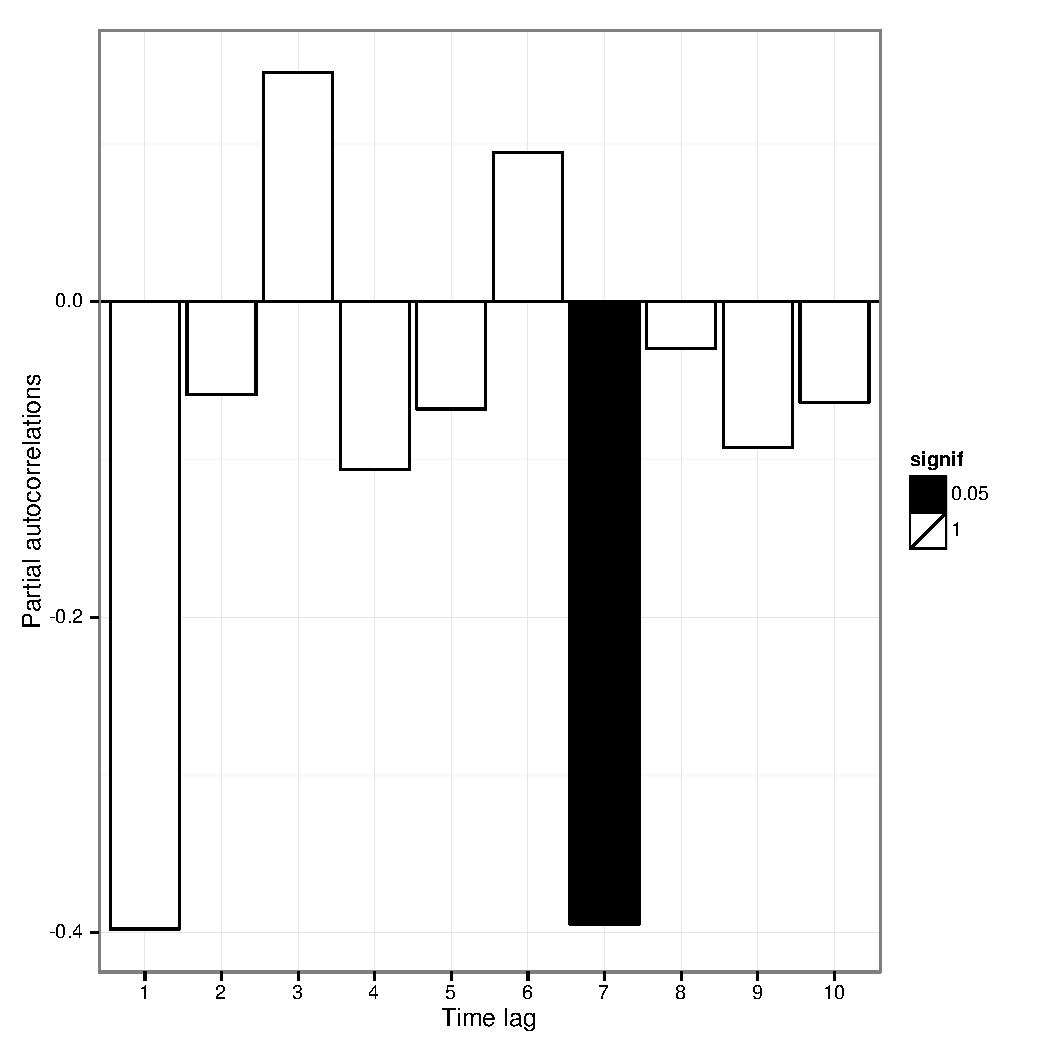
\includegraphics[width=65mm]{../White_Sea/dynamic_N_N1/perm_PRCF_Estuary_detrend.pdf}

	\end{center}
	\end{minipage}
		\hfil %Это пружинка отодвигающая рисунки друг от друга
	\begin{minipage}[b]{.46\linewidth}
%Следующий рисунок - первый ряд справа %DUNGEON S_4 \ AB
	\begin{center}
	{\footnotesize о.~Горелый}
		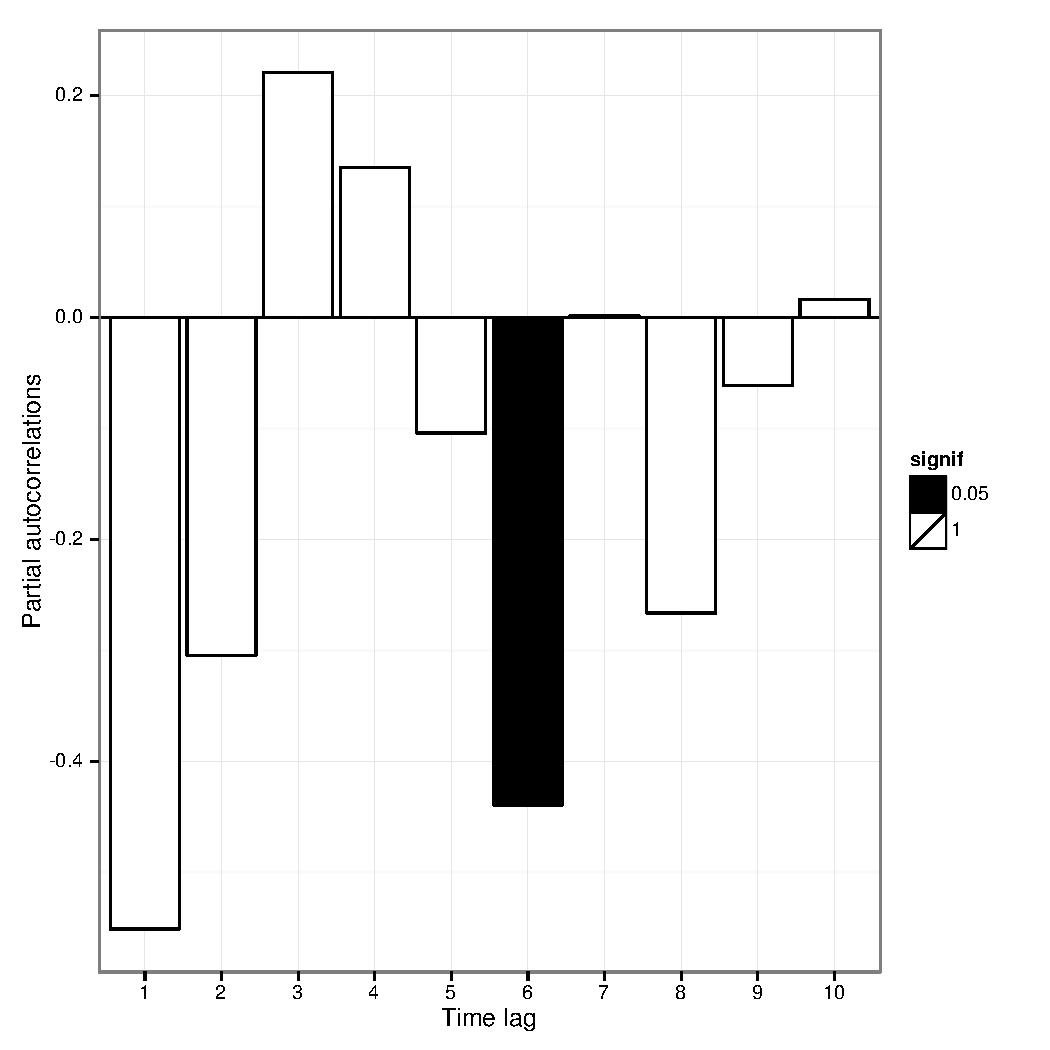
\includegraphics[width=65mm]{../White_Sea/dynamic_N_N1/perm_PRCF_Goreliy_all_detrend.pdf}
	\end{center}
	\end{minipage}

	\begin{minipage}[b]{.46\linewidth}
%Фигурка в первом ряду слева размер отведенный под весь этот объект \textendash 0.46 от ширины строки
%Параметр [b] означает, что выравнивание этих министраниц будет по нижнему краю
	\begin{center}
	{\footnotesize материковая литораль (Лувеньга)}
	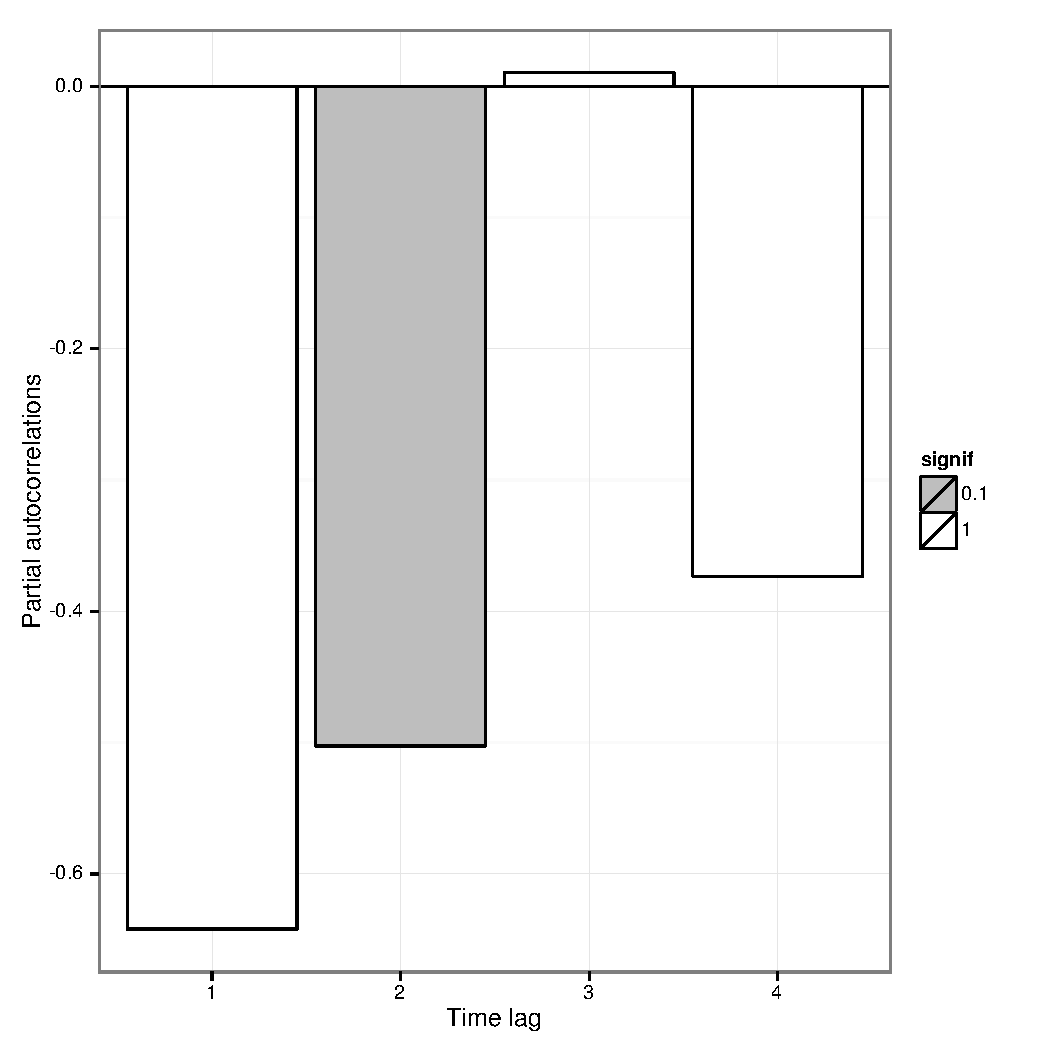
\includegraphics[width=65mm]{../White_Sea/dynamic_N_N1/perm_PRCF_razrez2_all_detrend.pdf}
	\end{center}
	\end{minipage}
		\hfil %Это пружинка отодвигающая рисунки друг от друга
	\begin{minipage}[b]{.46\linewidth}
%Следующий рисунок - первый ряд справа %DUNGEON S_4 \ AB
	\begin{center}
	{\footnotesize о.~Ломнишный}
	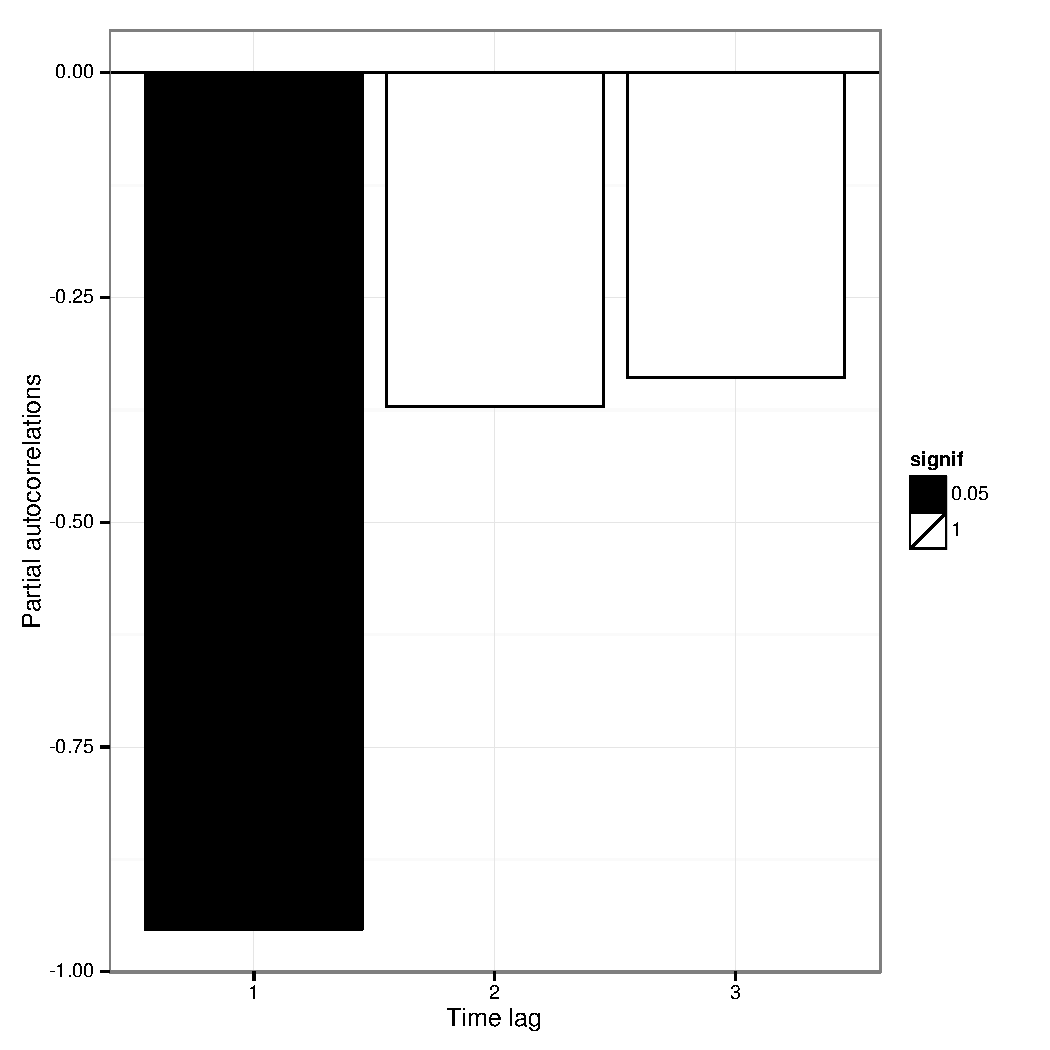
\includegraphics[width=65mm]{../White_Sea/dynamic_N_N1/perm_PRCF_Lomnishniy_detrend.pdf}
	\end{center}
	\end{minipage}

	\begin{minipage}[b]{.46\linewidth}
%Фигурка в первом ряду слева размер отведенный под весь этот объект \textendash 0.46 от ширины строки
%Параметр [b] означает, что выравнивание этих министраниц будет по нижнему краю
	\begin{center}
	{\footnotesize Южная губа о.~Ряшкова}
	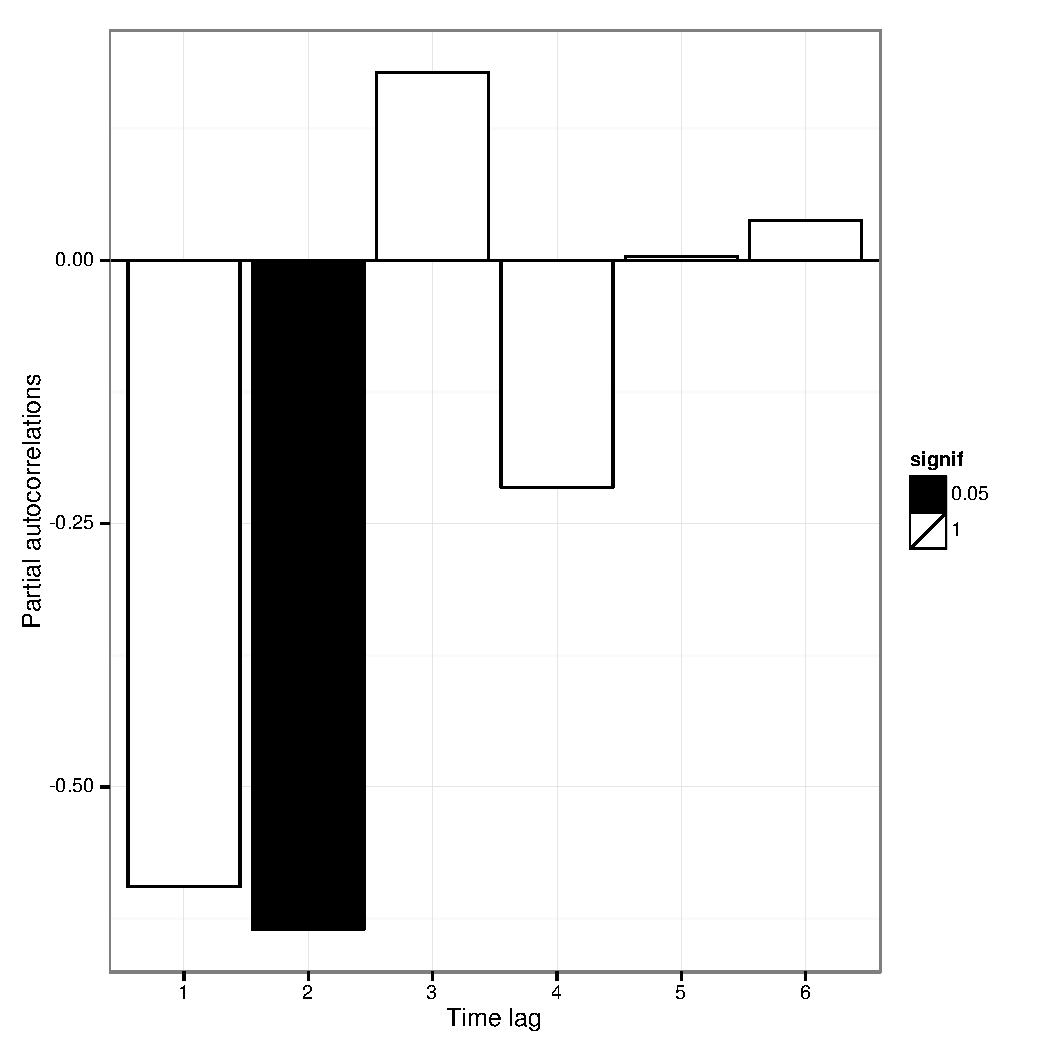
\includegraphics[width=65mm]{../White_Sea/dynamic_N_N1/perm_PRCF_YuG_detrend.pdf}
	\end{center}
	\end{minipage}
		\hfil %Это пружинка отодвигающая рисунки друг от друга
	\begin{minipage}[b]{.46\linewidth}
	\begin{center}	
	{\footnotesize Западная Ряшкова салма}
	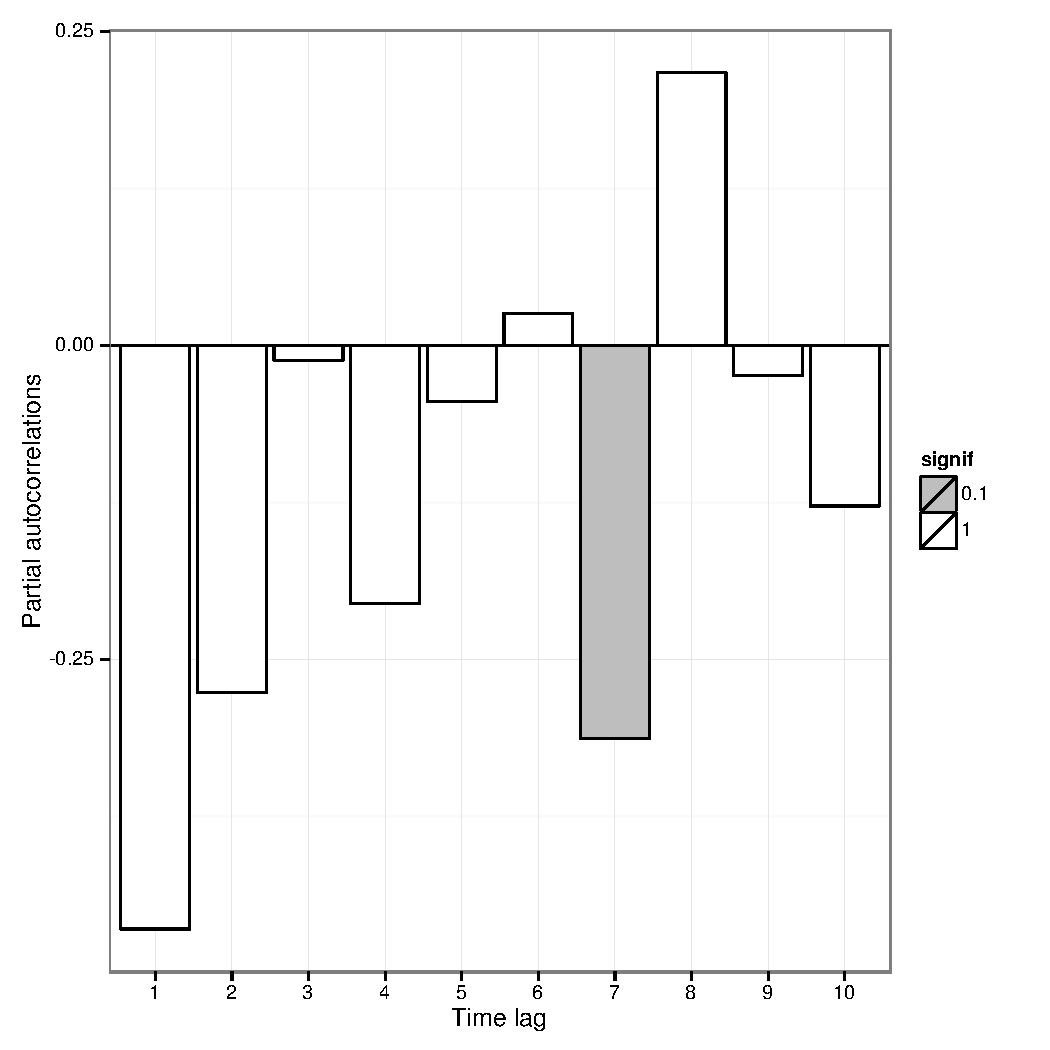
\includegraphics[width=65mm]{../White_Sea/dynamic_N_N1/perm_PRCF_ZRS_detrend.pdf}
	\end{center}
	\end{minipage}
	\caption{Частные корреляции плотности поселения {\it Macoma balthica} (без учета особей длиной менее 1 мм) в Кандалакшском заливе. Детрендированные данные. Оценка достоверности пермутационным методом.}
	\label{ris:perm_PRCF_Kandalaksha_N2_detrend}	
	\end{figure}

	\begin{figure}[p]
%\smallskip

	\begin{minipage}[b]{.46\linewidth}
%Фигурка в первом ряду слева размер отведенный под весь этот объект \textendash 0.46 от ширины строки
%Параметр [b] означает, что выравнивание этих министраниц будет по нижнему краю
	\begin{center}
	{\tiny Медвежья}
	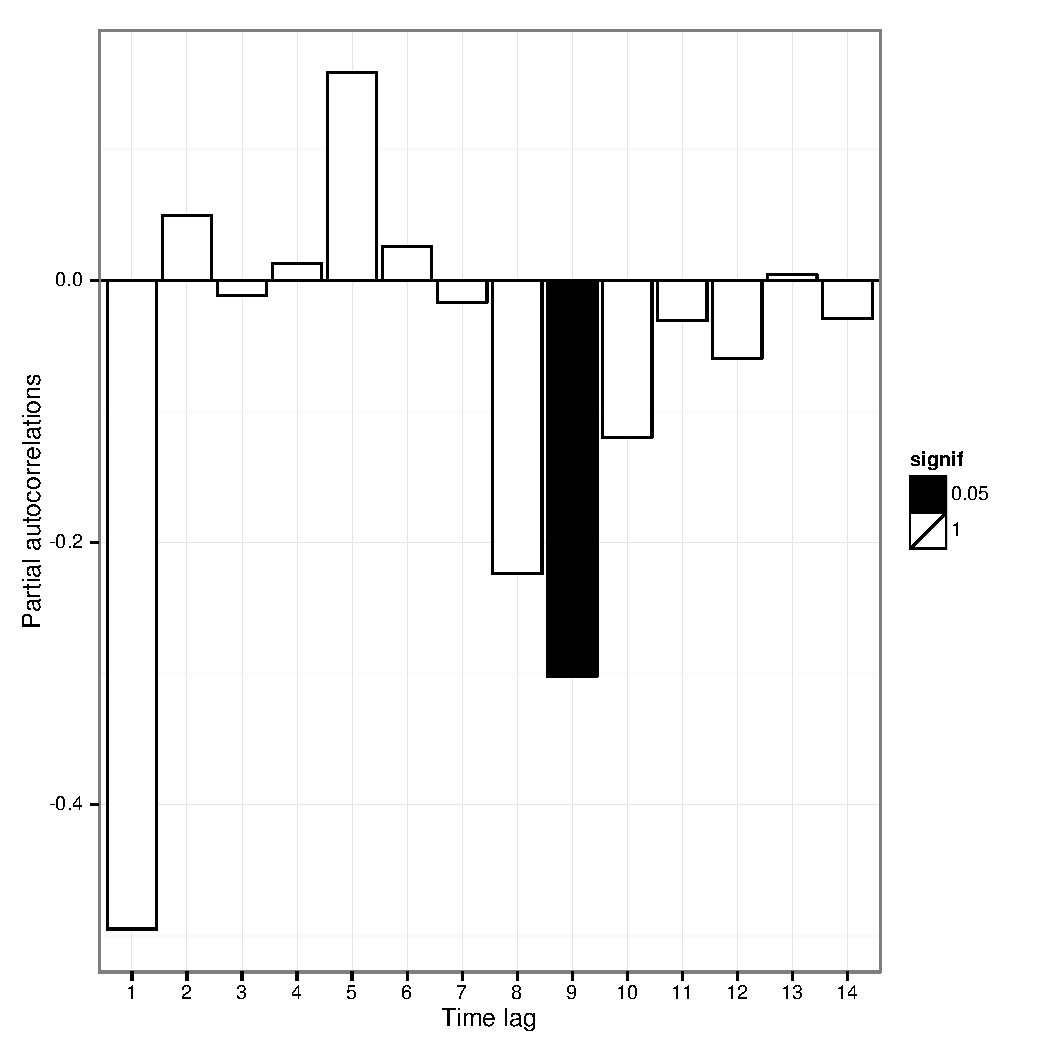
\includegraphics[width=65mm]{../White_Sea/dynamic_N_N1/perm_PRCF_Medvezhya_detrend.pdf}
	\end{center}
	\end{minipage}
%
	\hfil %Это пружинка отодвигающая рисунки друг от друга
%
	\begin{minipage}[b]{.46\linewidth}
	\begin{center}
	{\tiny Сельдяная}
	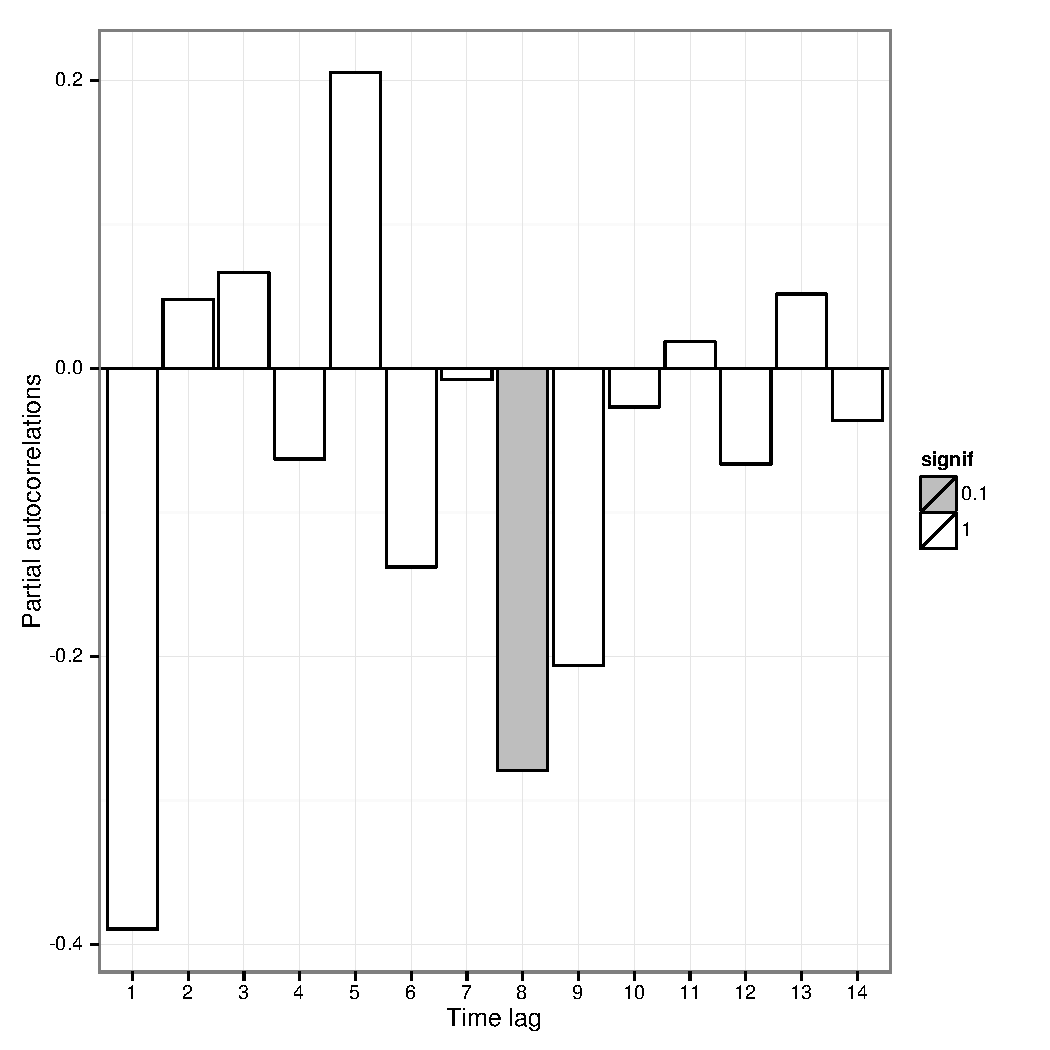
\includegraphics[width=65mm]{../White_Sea/dynamic_N_N1/perm_PRCF_Seldyanaya_detrend.pdf}
	\end{center}
	\end{minipage}

%\smallskip
%	\caption{Динамика плотности поселений {\it Macoma balthica} в вершине Кандалакшского залива}
%	\label{ris:dynamic_Kandalaksha_all}
\begin{center}
Рисунок \ref{ris:perm_PRCF_Kandalaksha_N2_detrend}, продолжение. Частные автокорреляции плотности поселения {\it Macoma balthica} (без учета особей длиной менее 1 мм) в Кандалакшском заливе. Детрендированные данные. Оценка достоверности пермутационным методом.
\end{center}
	\end{figure}
Для большинства временных рядов значение максимального значения достигает $PRCF$ с лагом 1, что характерно для динамики в отсутствие тренда. 
Достоверность частных автокорреляций оценивалась пермутационным методом.
Для участков в Южной губе о.~Ряшкова и на материковой литорали в Лувеньге были показаны достоверные значений $PRCF[2]$, причем в Южной губе $PRCF[2] > PRCF[1]$. 
Это показывает наличие в поселении плотностнозависимых процессов второго порядка.
Предположительно, это может быть воздействие хищников.
Мы надеемся проверить эту гипотезу в ходе дальнейших наблюдений.
Биологическая интерпретация $PRCF$ с большим лагом на настоящий момент представляется нам сомнительной.

		\subsection{Синхронность динамики плотности поселений {\it Macoma balthica} в Кандалакшском заливе Белого моря}
Для изучения синхронности колебаний плотности поселений маком мы использовали тест Мантеля.
Для включения большего количества рядов в анализ, он был проведен по двум наборам данных.
Первый набор данных включал участки, где при отборе проб промывка была на сите с диаметром ячеи $0,5$~мм. 
Сюда вошли участки в эстуарии р.~Лувеньги, на материковой литорали в районе Лувеньги, на о.~Горелый, в Западной Ряшковой салме и в губах Медвежья и Сельдяная (данные по последним двум губам взяты из работы \cite{Varfolomeeva_Naumov_2013}).
Результаты корреляционного анализа представлены в таблице~\ref{tab:Mantel_dynamic_N}.
	\begin{table}[p]
	\caption{Синхронность динамики плотности поселений {\it Macoma balthica}}
	\label{tab:Mantel_dynamic_N}
        \begin{tabularx}{\textwidth}{|p{0.2\textwidth}|*{6}{X|}} \hline
	$Mantel \ r \setminus p_{perm}$ & [1] & [2] & [3] & [4] & [5] & [6]   \\ \hline
            [1] эстуарий р.~Лувеньги            &         & \cellcolor{yellow}{ 0,002 }   & \cellcolor{yellow}{ 0,009 }     & \cellcolor{yellow}{ 0,001 }   &  0,264       &  0,441  \\ \hline
            [2] о.~Горелый              & \cellcolor{yellow}{ 0,929 }   &         & \cellcolor{yellow}{ 0,014 }     & \cellcolor{yellow}{ 0,001 }   &  0,388       &  0,089  \\ \hline
            [3] г.~Медвежья             & \cellcolor{yellow}{ 0,821 }   & \cellcolor{yellow}{ 0,86 }    &           & \cellcolor{yellow}{ 0,001 }   &  0,184       &  0,441  \\ \hline
            [4] материковая литораль (Лувеньга) & \cellcolor{yellow}{ 0,781 }   & \cellcolor{yellow}{ 0,784 }   & \cellcolor{yellow}{ 0,704 }     &         & \cellcolor{yellow}{ 0,044 }      &  0,123  \\ \hline
            [5] г.~Сельдяная            &  0,089    &  -0,009   &  0,087      & \cellcolor{yellow}{ 0,364 }   &            &  0,818  \\ \hline
%	[6] Западная Ряшкова салма  &  -0,045   &  0,057    &  -0,05      &  0,284    &  -0,141      &       \\ \hline
	\end{tabularx}
	   {\footnotesize Примечание: Нижняя половина таблицы --- значение теста Мантеля, верхняя половина --- уровень значимости, определенный пермутационным методом. \\
Выделены значения с уровнем значимости $< 0,1$. \\
$NA$ --- ряды не пересекаются во времени.}
	\end{table}
Три участка в районе Лувеньгских шхер (эстуарий р.~Лувеньги, о.~Горелый, материковая литораль) демонстрировали синхронную динамику поселений.
С данными участками была синхронна динамика поселения маком в г.~Медвежья. 
Низкая, хотя и достоверная корреляция была показана между динамикой на материковой литорали в районе Лувеньги и в г.~Сельдяной ($0,36$).


Второй набор данных включал участки, где при отборе проб промывку проводили на сите с диаметром ячеи $1$~мм.
Также сюда вошли те участки из предыдущего набора данных, где была известна размерная структура моллюсков --- из общей плотности поселения были вычтены обилие особей длиной менее $1$~мм для возможности сравнения.
Всего в данный анализ вошло 8 рядов данных: эстуарий р.~Лувеньги, материковая литораль в районе Лувеньги, о.~Горелый, Западная Ряшкова салма, Южная губа о.~ Ряшкова, о.~Ломнишный, б.~Клющиха и Сухая салма (данные по последним двум участкам взяты из работ \cite{Maximovich_et_al_1991, Maximovich_Gerasimova_2004, Gerasimova_Maximovich_2013}) (табл.~\ref{tab:Mantel_dynamic_N2}).
	\begin{table}[p]
	\caption{Синхронность динамики плотности поселения {\it Macoma balthica}.}
	\label{tab:Mantel_dynamic_N2}
        \begin{tabularx}{\textwidth}{|p{0.2\textwidth}|*{8}{X|}} \hline
	$Mantel \ r \setminus p_{perm}$ & [1] & [2] & [3] & [4] & [5] & [6] & [7] & [8]
	\\ \hline
	[1] эстуарий р.~Лувеньги & & $0,082$ & $0,646$ & $0,995$ & \cellcolor{yellow}{$0,029$} & $0,482$ & \cellcolor{yellow}{$0,013$} & $0,19$
	\\ \hline
	[2] о.~Горелый & $0,176$ &  & $0,067$ & $0,73$ & \cellcolor{yellow}{$0,001$} & $0,261$ & $0,986$ & \cellcolor{yellow}{$0,001$}
	\\ \hline
	[3] б.~Клющиха & $-0,046$ & $0,52$ &  & $0,673$ & \cellcolor{yellow}{$0,034$} & $0,213$ & $0,062$ & $0,065$
	\\ \hline
	[4] о.~Ломнишный & $-0,451$ & $-0,181$ & $-0,22$ &  & $NA$ & $1$ & $0,088$ & $0,341$
	\\ \hline
	[5] материковая литораль (Лувеньга) & \cellcolor{yellow}{$0,32$} & \cellcolor{yellow}{$0,862$} & \cellcolor{yellow}{$0,577$} & $NA$ &  & $0,117$ & $NA$ & \cellcolor{yellow}{$0,006$}
	\\ \hline
	[6]Сухая салма & $-0,019$ & $0,067$ & $0,085$ & $-1$ & $0,443$ &  & $0,688$ & $0,314$
	\\ \hline
	[7] Южная губа о.~ Ряшкова & \cellcolor{yellow}{$0,419$} & $-0,332$ & $0,434$ & $0,333$ & $NA$ & $-0,243$ &  & $0,605$
	\\ \hline
	[8] Западная Ряшкова салма & $0,114$ & \cellcolor{yellow}{$0,86$} & $0,72$ & $0,093$ & \cellcolor{yellow}{$0,755$} & $0,088$ & $-0,048$ & 
	\\ \hline
	\end{tabularx}
	   {\footnotesize Примечание: Нижняя половина таблицы --- значение теста Мантеля, верхняя половина --- уровень значимости, определенный пермутационным методом. \\
Выделены значения с уровнем значимости $< 0,05$. \\
$NA$ --- ряды не пересекаются во времени.}
	\end{table}
Интересно отметить, что при редукции данных до плотности поселений особей длиной более $1$~мм картина меняется.
Без изменения остается синхронность динамик поселений маком на материковой литорали в Лувеньге c о.~Горелый и эстуарием р.~Лувеньги.
Также сохраняется синхронность динамик плотности поселений в поселениях в эстуарии р.~Лувеньга и Южной губе о.~Ряшкова.
В то же время поселение в Западной Ряшковой салме, который в предыдущем анализе показывало асинхронность по сравнению с остальными участками, в данном случае демонстрирует синхронность с поселениями на о.~Горелый и материковой литорали в Лувеньге.
Также показана синхронность динамик поселений на материковой литорали в Лувеньге и в бухте Клющиха.

Мы использовали значение теста Мантеля как меру сходства рядов данных для тестирования гипотезы, что на более близко расположенных участках динамика плотности поселений {\it Macoma balthica} более сходна.
Для этого по координатам участков была рассчитана матрица расстояний между участками (табл.~\ref{tab:distance_area_km}).
	\begin{table}[p]
	\caption{Расстояние между исследованными участками литорали.}
	\label{tab:distance_area_km}
        \begin{tabular}{|p{0.3\textwidth}|*{10}{p{0.04\textwidth}|}} \hline
	 & [1] & [2] & [3] & [4] & [5] & [6] & [7] & [8] & [9] & [10]
	\\ \hline
	[1] материковая литораль (Лувеньга) & 0,0 &  &  &  &  &  &  &  &  & 
	\\ \cline{1-3}
	[2] о.~Горелый & 1,5 & 0,0 &  &  &  &  &  &  &  &  
	\\ \cline{1-4}
	[3]эстуарий р.~Лувеньги & 1,0 & 1,0 & 0,0 &  &  &  &  &  &  &  
	\\ \cline{1-5}
	[4] Южная губа о.~Ряшкова & 11,7 & 10,7 & 11,7 & 0,0 &  &  &  &  &  & 
	\\ \cline{1-6}
	[5] о.~Ломнишный & 13,5 & 12,9 & 13,8 & 3,7 & 0,0 &  &  &  &  &  
	\\ \cline{1-7}
	[6] Западная Ряшкова салма & 11,9 & 10,8 & 11,8 & 1,7 & 5,3 & 0,0 &  &  &  &  
	\\ \cline{1-8}
	[7] г.~Сельдяная & 93,6 & 94,0 & 94,5 & 87,8 & 84,1 & 89,3 & 0,0 &  &  &  
	\\ \cline{1-9}
	[8] г.~Медвежья & 91,9 & 92,4 & 92,8 & 86,1 & 82,4 & 87,6 & 1,7 & 0,0 &  &  
	\\ \cline{1-10}
	[9] Сухая салма & 97,1 & 97,5 & 97,9 & 91,2 & 87,6 & 92,7 & 3,5 & 5,1 & 0,0 &  
	\\ \hline
	[10] б.~Клющиха & 100,1 & 100,6 & 101,0 & 94,8 & 91,1 & 96,3 & 8,1 & 9,7 & 5,8 & 0,0
	\\ \hline
	\end{tabular}
	   {\footnotesize Примечание:Расстояние дано в километрах.}
	\end{table}

Для обоих наборов данных тест Мантеля показал отсутствие зависимости сходства динамики плотности поселений маком от расстояния ( $Mantel\ r = --0,058 (p_{perm} = 0,746)$ и $Mantel\ r = -0,105 (p_{perm} = 0,638)$ для первого и второго набора данных, соответственно).

\afterpage{\clearpage}
